% This is a template to create your midterm report as a pdf.
% Just fill in the areas and run pdflatex
% For more information on LaTeX documents consult The (Not So
% Short Introduction to LateX2e
%
% to compile your report use the command
% pdflatex midtermreport.tex
%
% if you have \ref useage or other cross links
% you will have to run the above command again

% set 12pt font
\documentclass[12pt]{article}
% some useful packages
\usepackage[pdftex]{graphicx,color}
\usepackage{fullpage}
\def\baselinestretch{1.5} % line spaceing
% set title
\title{Midterm Design Report \\
	ECE 437L}
% fill in the blanks
\author{Yutong Huang, Yiheng Chi \\
        John Skubic, Noah Chesnut, Abhishek Srikanth}
% \today will put todays date
% or you can manually put the date in
\date{Mar. 3, 2017}
% cover page is a page by itself

\begin{document}
  \maketitle

  \newpage
% executive overview remember
% this should be on a page by itself
  \section{Executive Overview}
  
  So far, single cycle processor design and pipeline processor design have been completed and carefully verified. In this report, we are going to compare pros and cons of each design including frequency, instruction CPI, total instruction execution time, and resource requirement. For controlling variables, comparison is performed under the same binary program which perform a merge sort algorithm. Merge sort is selected since it contains a lot of branch instructions, heavy dependency of each instruction, and frequent load use. Combination of hazards happened is helpful for design verification and related large number of dynamic instruction differentiate two designs more clearly. \\
  In general, single cycle design uses less gate resources, since every instruction is executed in only one cycle, no any dependency relevant problems will happened. Inversely, pipeline design requires much more resources including pipeline registers and combinational logic gates used for resolving various hazard, but low critical path between each pipeline makes a higher clock frequency possible. In total, based on testing result, pipeline design will execute program much faster and consume more resources simultaneously.

  \newpage
  \section{Processor Design}

% Uncomment after you create the block diagram graphic.
  \begin{figure}[hp]
    \begin{center}
      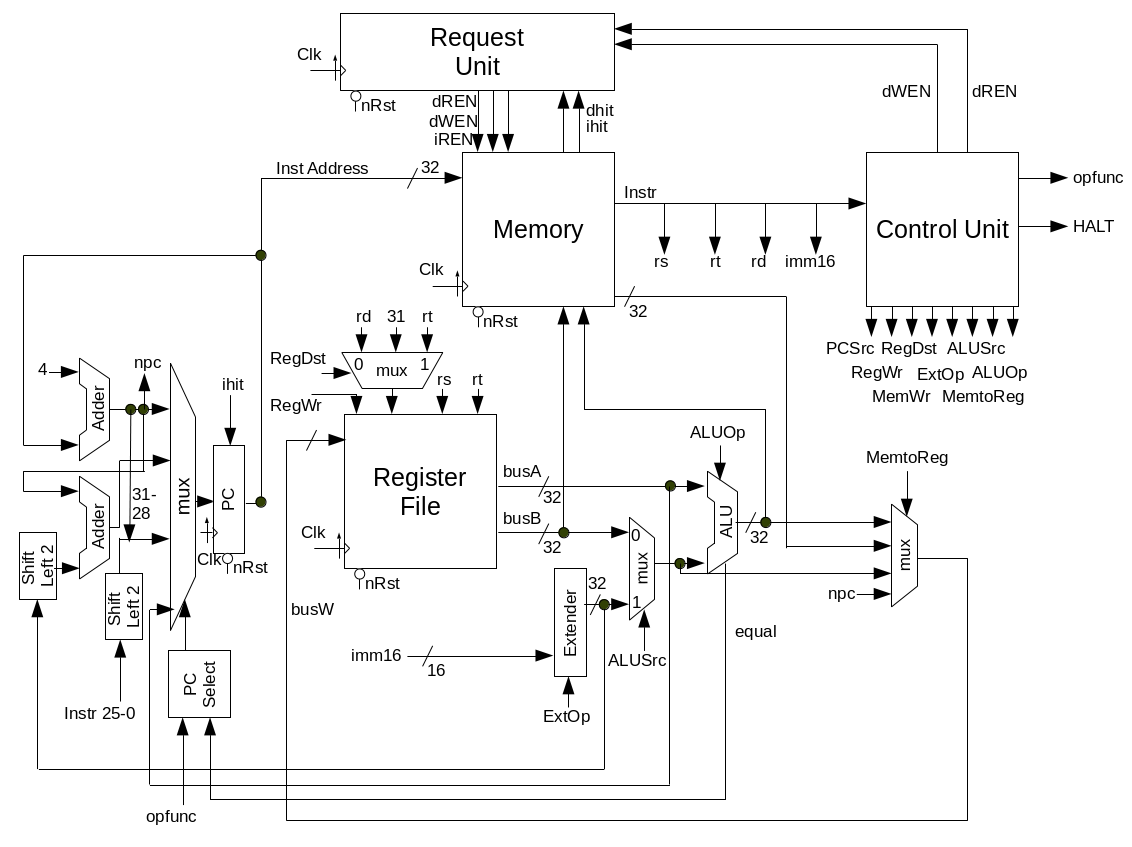
\includegraphics[width=\textwidth]{diagram_singlecycle.png}
    % You can change the type of figure to a .png, .pdf, .jpg, .mps
    \end{center}

    \caption{Single Cycle Block Diagram}
		\label{fig:singlecycle}
  \end{figure}

  \newpage
  \begin{figure}[hp]
    \begin{center}
      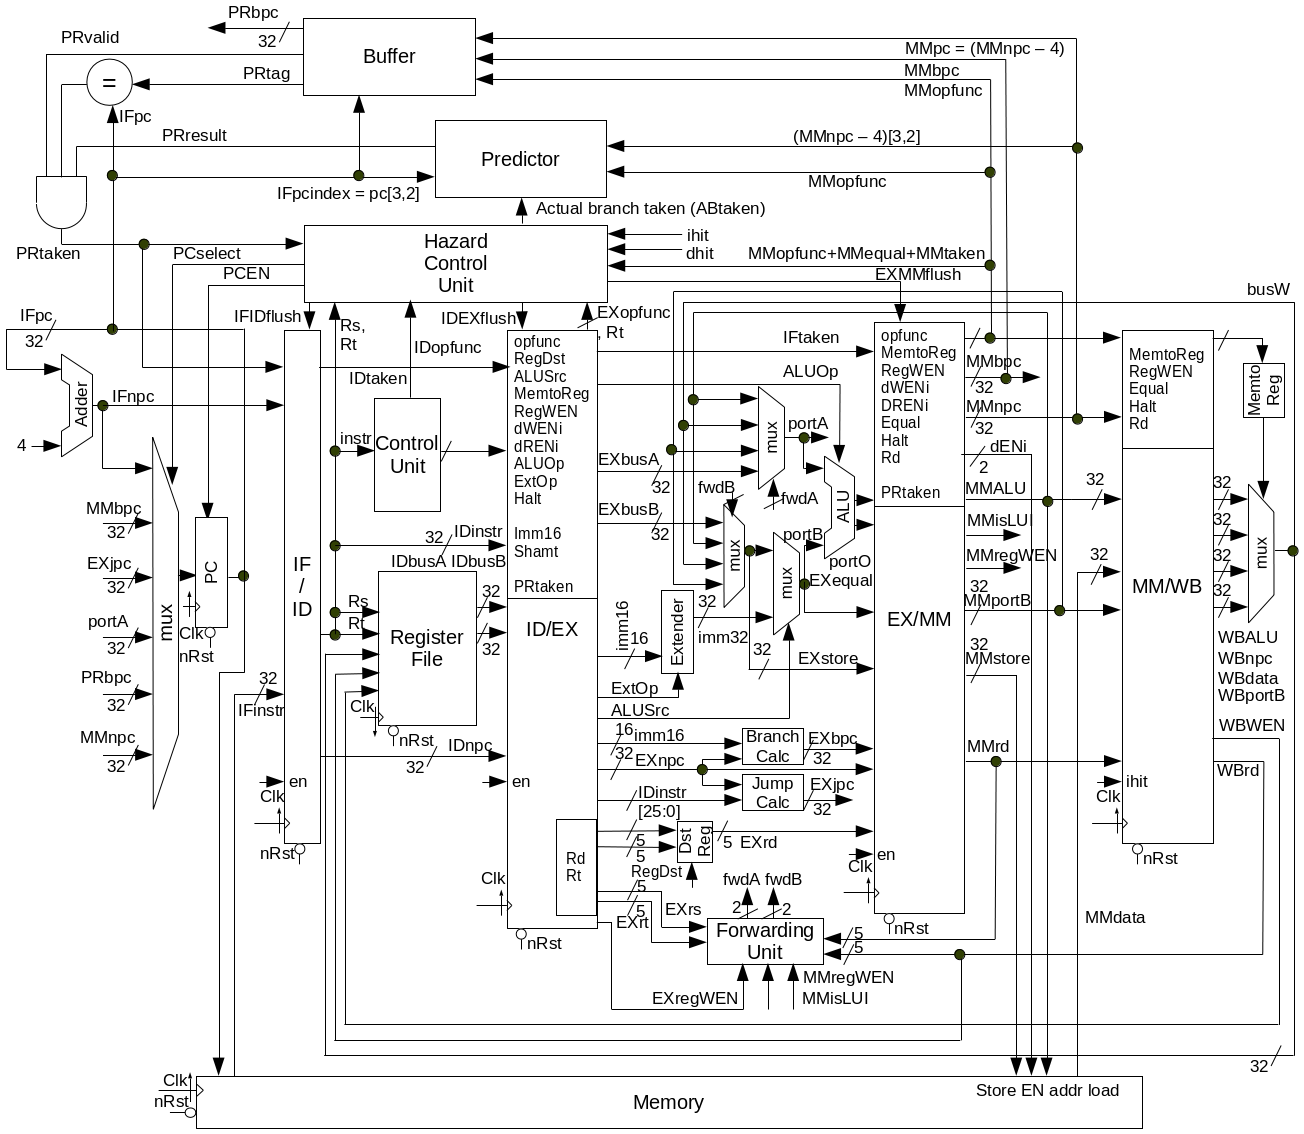
\includegraphics[width=\textwidth]{diagram_pipeline.png}
    % You can change the type of figure to a .png, .pdf, .jpg, .mps
    \end{center}

    \caption{Pipeline Block Diagram}
		\label{fig:pipeline}
  \end{figure}

  %Text for discussing your designs in Figure \ref{fig:processor}
  \newpage
  \section{Results}

  \begin{table}[!hbp]

    \begin{tabular}{|p{.42\textwidth}|p{.25\textwidth}|p{.25\textwidth}|}
      \hline
       & Single Cycle Processor & Pipeline Processor \\ \hline
      Frequency of design: & -- & -- \\ \hline
      - Max possible frequency from logs & 35.42 MHz & 64.04 MHz \\ \hline
      - Highest frequency achieved from tb & 25 MHz & 25 MHz \\ \hline
      Average instructions per clock cycle & 0.7829 & 0.6191 \\ \hline
      Latency of one instruction & 28.233 ns & 78.076 ns \\ \hline
      Total execution time of the program & 389.38 ms & 272.46 ms \\ \hline
      FPGA resources required for design: & -- & -- \\ \hline
      - Total combinational functions & 2918 & 3521 \\ \hline
      - Total registers & 1285 & 2032 \\ \hline
    \end{tabular}

    \caption{Processor Specs}
		\label{tb:procspec}
  \end{table}
  Max possible frequency of design is obtained from the system log which show the restricted Fmax in the ``Slow 1200mV 85C Model Fmax Summary'' section. In this section CLK and CPUCLK frequencies are given and the max possible frequency should be min(CLK/2, CPUCLK). Highest frequency achieved are calculated based on the smallest clock period, which is obtained by repeatedly testing designs under different clock period in an ascendant order specified in system test benches until the design breaks. The highest frequency equals 1/(Smallest clock period). The total number of instructions is obtained from running a ``sim'' command which reports it at the end, and the total clock cycles running the program is obtained from running a ``make system.sim'' command which also reports at the end. The average instruction per clock cycle is (Total number of instructions)/(Total clock cycles). Latency of one instruction is 1/(Max possible frequency) for single cycle processor and 5/(Max possible frequency) for pipeline. Total execution time of the program is (Clock period)*(Total clock cycles). FPGA resources required are found in system FPGA log file in the “Fitter Summary” section.

  \section{Conclusion}

  Based on the result above, pipeline design has a higher maximum frequency than single cycle does. However, in real testing, pipeline design cannot achieve these frequency and run a clock speed closed to single cycle design to single at 25 MHz. The 5 stages of pipeline results a higher latency per instruction in pipeline design but not really 5 times higher. Therefore, with benefit that pipeline design can hold 5 instructions at the same time, pipeline design has a lower total execution time. \\ About resource usage, both combinational gates and registers used are higher in pipeline design. Registers used is significantly high in pipeline since each pipe transfer almost all the signals from current stages to next stage which requires a lot of registers to carry these signals. Besides pipeline registers, branch prediction buffers also require a relatively large amount of registers to store target register and state machine. For combinational logic, the use of forwarding unit, hazard unit and branch prediction consumes most of extra combinational block compared to single cycle design. Trivial combinational logic goes to muxes modified from single cycle design. In conclusion, same program run by pipeline design is faster than run by single cycle and pipeline design requires more resources


  \section{Contributions}

  Yutong Huang: Complete single cycle processor, datapath modification and integration, pipe flip-flops implementation, branch prediction state machine, branch predictor diagram, overall design testing and debugging, midterm report overview and conclusion section. \\ \\
  Yiheng Chi: Complete single cycle processor, forwarding unit implementation, hazard control unit implementation, branch prediction buffer implementation, early stage pipeline design and diagram drawing, overall design testing and debugging, midterm report processor design and result section.

\end{document}
